% ClaimTrace architecture figure. Compile with pdfLaTeX (Overleaf: New Project -> Blank, paste, Recompile).
\documentclass[tikz,border=10pt]{standalone}
\usepackage[T1]{fontenc}
\usepackage{lmodern}
\usetikzlibrary{positioning,arrows.meta,fit,calc}

\begin{document}
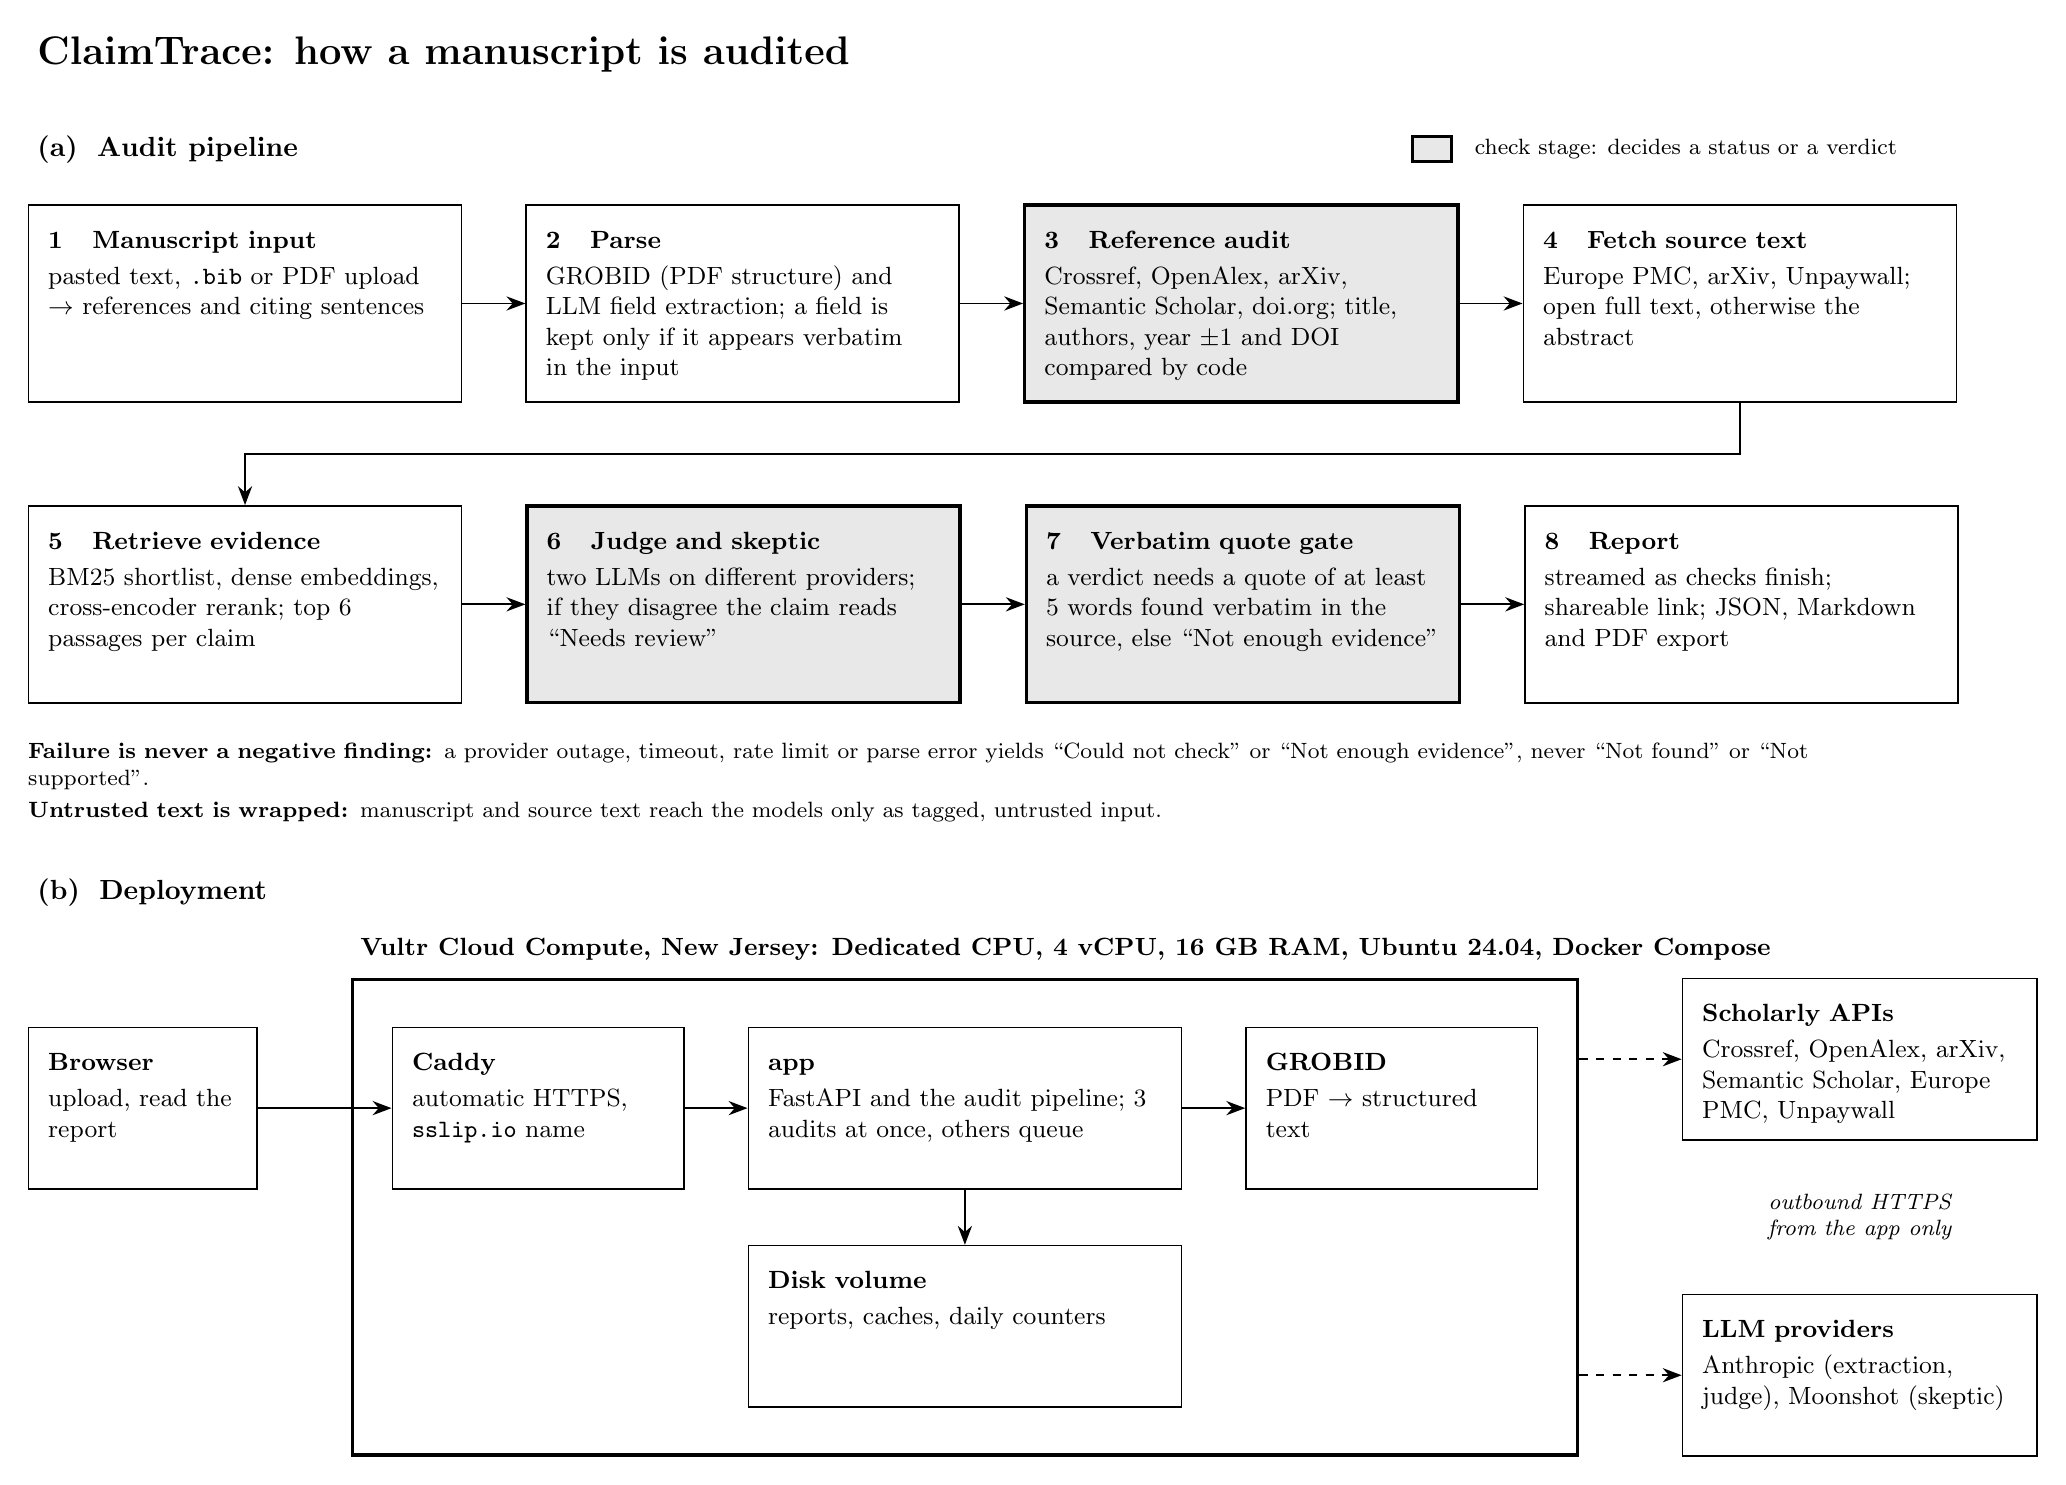
\begin{tikzpicture}[
  font=\small,
  >={Stealth[length=2.4mm,width=1.8mm]},
  node distance=8mm,
  box/.style={draw, line width=0.6pt, rectangle, align=left, text width=50mm,
              text height=3mm, text depth=17mm, inner sep=2.5mm,
              execute at begin node={\hyphenpenalty=10000\exhyphenpenalty=10000}},
  chk/.style={box, fill=black!9, line width=1.2pt},
  small/.style={box, text depth=12.5mm},
  flow/.style={->, line width=0.7pt},
  ext/.style={->, line width=0.7pt, dashed},
  hd/.style={font=\normalsize\bfseries, anchor=west},
]

% ---------- (a) audit pipeline ----------
\node[box] (n1) {\textbf{1\quad Manuscript input}\\[2pt]
  pasted text, \texttt{.bib} or PDF upload\\
  $\rightarrow$ references and citing sentences};
\node[box, right=of n1] (n2) {\textbf{2\quad Parse}\\[2pt]
  GROBID (PDF structure) and LLM field extraction; a field is kept only
  if it appears verbatim in the input};
\node[chk, right=of n2] (n3) {\textbf{3\quad Reference audit}\\[2pt]
  Crossref, OpenAlex, arXiv, Semantic Scholar, doi.org; title, authors,
  year $\pm 1$ and DOI compared by code};
\node[box, right=of n3] (n4) {\textbf{4\quad Fetch source text}\\[2pt]
  Europe PMC, arXiv, Unpaywall; open full text, otherwise the abstract};

\node[box, below=13mm of n1] (n5) {\textbf{5\quad Retrieve evidence}\\[2pt]
  BM25 shortlist, dense embeddings, cross-encoder rerank; top 6 passages
  per claim};
\node[chk, right=of n5] (n6) {\textbf{6\quad Judge and skeptic}\\[2pt]
  two LLMs on different providers; if they disagree the claim reads
  ``Needs review''};
\node[chk, right=of n6] (n7) {\textbf{7\quad Verbatim quote gate}\\[2pt]
  a verdict needs a quote of at least 5 words found verbatim in the source,
  else ``Not enough evidence''};
\node[box, right=of n7] (n8) {\textbf{8\quad Report}\\[2pt]
  streamed as checks finish; shareable link; JSON, Markdown and PDF export};

\draw[flow] (n1) -- (n2);
\draw[flow] (n2) -- (n3);
\draw[flow] (n3) -- (n4);
\draw[flow] (n4.south) -- ++(0,-6.5mm) -| (n5.north);
\draw[flow] (n5) -- (n6);
\draw[flow] (n6) -- (n7);
\draw[flow] (n7) -- (n8);

\node[hd] (ha) at ($(n1.north west)+(0,7mm)$) {(a)\; Audit pipeline};
\node[anchor=west, font=\Large\bfseries] at ($(n1.north west)+(0,19mm)$)
  {ClaimTrace: how a manuscript is audited};
\node[draw, line width=1.2pt, fill=black!9, minimum width=5mm, minimum height=3.2mm,
      inner sep=0pt, anchor=east] (lg) at ($(n4.north east)+(-64mm,7mm)$) {};
\node[anchor=west, font=\footnotesize] at ($(lg.east)+(1.5mm,0)$)
  {check stage: decides a status or a verdict};

\node[anchor=north west, align=left, text width=240mm, font=\footnotesize,
      inner sep=0pt] (notes) at ($(n5.south west)+(0,-5mm)$) {%
  \hyphenpenalty=10000\exhyphenpenalty=10000
  \textbf{Failure is never a negative finding:} a provider outage, timeout,
  rate limit or parse error yields ``Could not check'' or ``Not enough
  evidence'', never ``Not found'' or ``Not supported''.\\[2pt]
  \textbf{Untrusted text is wrapped:} manuscript and source text reach the
  models only as tagged, untrusted input.};

% ---------- (b) deployment ----------
\node[hd] (hb) at ($(notes.south west)+(0,-9mm)$) {(b)\; Deployment};

\node[small, text width=24mm, anchor=north west] (br)
  at ($(hb.south west)+(0,-14mm)$) {\textbf{Browser}\\[2pt] upload, read the report};
\node[small, text width=32mm, right=17mm of br] (caddy)
  {\textbf{Caddy}\\[2pt] automatic HTTPS, \texttt{sslip.io} name};
\node[small, text width=50mm, right=of caddy] (app)
  {\textbf{app}\\[2pt] FastAPI and the audit pipeline; 3 audits at once, others queue};
\node[small, text width=32mm, right=of app] (grobid)
  {\textbf{GROBID}\\[2pt] PDF $\rightarrow$ structured text};
\node[small, text width=50mm, below=7mm of app] (vol)
  {\textbf{Disk volume}\\[2pt] reports, caches, daily counters};

\node[draw, line width=1.2pt, fit=(caddy)(app)(grobid)(vol), inner sep=5mm,
      inner ysep=6mm] (vultr) {};
\node[anchor=south west, font=\small\bfseries] at ($(vultr.north west)+(0,1mm)$)
  {Vultr Cloud Compute, New Jersey: Dedicated CPU, 4 vCPU, 16 GB RAM, Ubuntu 24.04, Docker Compose};

\node[small, text width=40mm, anchor=north west] (apis)
  at ($(vultr.north east)+(13mm,0)$)
  {\textbf{Scholarly APIs}\\[2pt] Crossref, OpenAlex, arXiv, Semantic Scholar, Europe PMC, Unpaywall};
\node[small, text width=40mm, anchor=south west] (llm)
  at ($(vultr.south east)+(13mm,0)$)
  {\textbf{LLM providers}\\[2pt] Anthropic (extraction, judge), Moonshot (skeptic)};

\draw[flow] (br) -- (caddy);
\draw[flow] (caddy) -- (app);
\draw[flow] (app) -- (grobid);
\draw[flow] (app) -- (vol);
\draw[ext] (vultr.east |- apis.west) -- (apis.west);
\draw[ext] (vultr.east |- llm.west) -- (llm.west);
\node[font=\footnotesize\itshape, align=center] at ($(apis.south)!0.5!(llm.north)$)
  {outbound HTTPS\\from the app only};
\end{tikzpicture}
\end{document}
